\chapter{Monocular Scale}

\section{Introduction}

Recovering camera 6-DOF ego-motion from images is a well studied
problem. It arises in various practical contexts
(e.g. virtual/augmented reality application, autonomous or aided
navigation, etc.).  The problem was studied in both stereo and the
monocular setups.  To recover the full 6-DOF motion, the previous
works resorted to the stereo setup, used auxiliary sensors (e.g. IMU)
or rely on the planar motion assumption.  All of these have their
drawbacks: stereo pairs are fragile and require careful calibration
procedures, additional sensors are not always available and also
require calibration, scene assumptions don't always hold.  Motion
estimation from images of a single moving camera is probably the
hardest setup, as well as the most desirable one, because of its
simplicity.  It is well known that the translation scale parameter is
not directly observable for a motion of a single camera.

We argue, that for natural scenes the scale information is present in
the images (see e.g. Figure~\ref{fig:feature_vectors}).  We propose to
apply statistical machine learning techniques to learn the monocular
scale.  We experiment with random forest, convolutional neural nets
and recurrent neural nets. In the following sections we present an
overview of the existing works in the field, describe our method and
present the experimental results.

\section{Related work}
\paragraph{Geometric methods} Previous geometric works in monocular
scale estimation may roughly be divided into ground plane and
non-ground plane methods.

Ground plane methods rely on the following assumptions: camera height
(a distance from the camera principle center to the ground plane) is
known to the method, a predefined region of the image (usually the one
in front of the camera in the world) contains projections of the
ground plane points, the ground is in front of the camera.  These
assumptions allow to properly scale the camera motion vector.

Ground planes in consecutive images are commonly related by a
homography matrix. Homography matrix may be estimated from a set of
sparse correspondences (e.g.,~\cite{song2014robust}) or from dense
region matching as in ~\cite{7995955}.  The sparse correspondence
method is sensitive both to outliers and to scarcity of features in
the ground region.  Dense region methods tend to fail when the region
deviates from being planar (especially in curb areas). Modern methods
parameterize the homography through camera and plane parameters rather
than plane matrix entries.  This allows to prevent homography
decomposition step that introduces additional errors, see
e.g.,~\cite{zhou2016reliable}, that contributes a divide-and-conquer
approach, where they decompose the ground plane homography into the
structure and the motion parameters.  Their optimization step is based
on this division.  ~\cite{kitt2011monocular} take a more SLAM-like
approach by collecting and keeping track of a constant number of
ground-plane features which they use to refine the scale.
~\cite{grater2015robust} complement the ground plane estimation based
on the structure from motion techniques with vanishing point
estimation which renders the algorithm robust in urban
scenarios. ~\cite{7995955} considers both dense and sparse cues for
ground plane estimation.  This makes their method robust toward
varying availability and distribution of trackable ground structure.
They parameterize and optimize over the motion parameters directly,
instead of optimizing the ground plane homography.  Furthermore they
use classifiers based on e.g., moments and residuals to reject scale
outliers.

The idea of using non-ground objects to estimate scale was explored
by~\cite{song2014robust} and~\cite{frost2016}.  These works employ
object size change as an additional cue to determine the correct scale.

Another category of works proceed by making assumptions on the camera
motion. In~\cite{gutierrez2012full} the authors assume head-mounted
camera and relate the vertical camera oscillation frequency to the step
length and, subsequently, to person height, which allows full 6DOF
motion estimation. ~\cite{scaramuzza2009absolute} assumes that the
vehicle adheres to the Ackerman steering principle and exploit the
non-holomicity of its motion, to compute the scale.

\paragraph{Learning methods} There are a number of works that use
machine learning approaches to solve the 6DOF visual odometry.
Optical flow is used to train k-nearest neighbor, Gaussian processes
and support vector machines in ~\cite{roberts2008memory},
~\cite{guizilini2013semi}, ~\cite{CIARFUGLIA20141717}
respectively. ~\cite{wang2017deepvo} shows that visual odometry may be
addressed in the end-to-end fashion, using the deep learning
techniques. The authors use CNN to learn the geometric feature
representation and the recurrent neural networks to model sequential
motion dynamics. In~\cite{muller2017flowdometry}, the authors use
optical flow images as CNN input to learn and infer camera
motion. Authors in~\cite{DBLP:journals/corr/MohantyADGSC16} also
propose to train a CNN.

Recent work of~\cite{frost2017using} (our work was done independently)
performs similar experiment to ours.  They train a convnet to predict
camera translation vector magnitude (referred to as ``speed'').  Their
work makes two major contributions: a method to learn a camera
``speed'' and a regularization method to incorporate such speed
prediction into a bundle adjustment procedure.  Their learning
procedure is very similar to the one proposed in this work.  The novel
regularization they propose penalizes differences between the
estimated and measured speed of the camera during the open-loop
trajectory. They are able to produce a virtually scale drift free
monocular SLAM trajectories using the combination of the above two
procedures.  We compare to their results.

\subsection{Our method}\label{sec:our method}

We assume that a single camera moves through space and takes images.
We treat the initial camera pose (at time $t=0$) as the world
coordinate frame.  We denote the pose of the camera at time $t$ by
$\mathbf{\hat{T}}_t$ described by the rotation matrix
$\mathbf{\hat{R}}_t$ and the translation vector $\mathbf{\hat{t}}_t$
as seen in the world coordinate frame.  We denote camera image taken
at time $t$ by $I_t$.  To facilitate the discussion, we also introduce
notation for camera pose
$\mathbf{T}_t = [\mathbf{R}_t\ |\ \mathbf{t}_t] $ as seen from the
coordinate frame associated with camera pose at time $t-1$.  Most of
the time, we will omit the time index, since its clear from the
context.  By translation scale (or simply, scale) we refer to the norm
of the translation vector $\mathbf{t}$ (e.g.,
$s = \lVert \mathbf{t} \rVert$)

We pose the scale estimation problem as a regression problem and
search for a good regressor model.  We evaluate random forest, two
different convnet architectures and a recurrent neural network.

\section{Random forest}

\subsection{Decision trees}

In this section we briefly describe tree-based methods for regression.
These involve splitting the feature space into a number of small
regions.  The prediction for a sample is made by computing a mean or a
mode of training samples that belong to the same region.  Since the
set of rules used to split the feature space into smaller regions may
be described by a tree, these methods are referred to as
\textit{decision tree} methods.

Building a decision tree may be described by a two step procedure:
\begin{enumerate}
\item Split the feature space, e.g., the set of all possible values
  for $X_1, X_2,\ldots,X_n$ into $J$ distinct regions $R_1, R_2,\ldots, R_J$.
\item For every sample that belongs to the regions $R_i$ we make the
  same prediction, which is a mean of the responses of training
  samples that belong to this region.
\end{enumerate}

The regions $R_i$ are usually chosen to be multidimensional boxes
(axis aligned).  We would like to find such a partition of the feature
space that minimizes
\begin{equation}\label{eq:tree_objective}
\sum\limits_{j=1}^J\sum_{x\in R_j}{(x-\mean{y}_j)^2},
\end{equation}

Where $y_j$ denotes the mean of the response values of the samples in
region $R_j$.  Unfortunately, solving the optimization
problem~\ref{eq:tree_objective} is computationally hard.  Usually it
is replaced with a greedy algorithm, called \textit{recursive binary
  splitting}.  This approach starts at the top of the tree and
greedily chooses the best split at that point that minimizes the
variance of its sub-trees.  To be more precise, for each $j$ and $s$
we define the hyper-planes:

\begin{equation}
  R_1(j,s) = \{ X\lvert X_j<s \}\quad\text{and}\quad R_2(j,s) = \{ X\lvert X_j \geq s \},
\end{equation}

We seek such $j$ and $s$ that minimize the equation:

\begin{equation}
  \sum\limits_{i:x_i\in R_1(j,s)}{(x_i-y_{R_1})}^2 + \sum\limits_{i:x_i\in R_2(j,s)}{(x_i-y_{R_2})}^2,
\end{equation}

Where $y_{R_1}, y_{R_2}$ are the average responses of the samples in
$R_1(j,s), R_2(j,s)$ respectively.  Once we found the $j$ and $s$ we
recursively split each sub-tree in a similar manner.  The process is
repeated until a stopping criterion (e.g., number of nodes in the
leaf) is reached.

\subsection{Bagging}
Decision trees tend to suffer from \textit{high variance}. This means
that if we split the training set into a number of random subsets and
fit random tree into each sub-sample, we would likely to get much
different answers from these trees when asked the same question.  It
is known that the variance of a mean of a set of independent random
variables is $\frac{1}{n}$.  Thus, in order to improve the variance of
the estimator, it is possible to fit $n$ estimators, each to its
training-set and the average their predictions.  Since, usually, we
don't have $n$ training sets, we would use \textit{bootstrapping}
(e.g., sample independently with replacement from the data set).

\subsection{Random Forest}
The random forest suggests an additional improvement over bagging, by
decorrelating the random trees.  The issue they attempt to address is
this: lets say there is a very dominant feature w.r.t. to task at hand
for a given data-set.  Bagging ensures that we use different training
sets, but yet, most trees will tend to first split on this dominant
feature.  In this case the trees will resemble each other.  In random
forest, the trees are constructed by using only a subset of features
(e.g., $m = \sqrt{p}$).  This means that at calculating the splits,
the algorithm is allowed to consider only a subset of features.

\section{Convolutional Neural Networks}

Convolutional neural networks (CNN) leverage the availability of the
computational power and the abundance of data.  CNN have become a
method of choice in a number of computer vision areas (e.g., image
classification~\cite{krizhevsky2012imagenet} ~\cite{simonyan2014very},
~\cite{szegedy2015going}, object recognition
~\cite{sermanet2013overfeat}~\cite{girshick2014rich}
~\cite{he2014spatial}.  They were also shown capable of per-pixel
tasks, such as semantic segmentation
~\cite{ning2005toward}~\cite{gupta2014learning}, depth estimation from
a single image ~\cite{liu2016learning}, optical flow
estimation~\cite{fischer2015flownet}.

Network architecture is a choice that needs to be made a priori.  To
best of our knowledge, there is no clear guideline on how to choose a
network architecture for a new task.  We experiment with two network architectures:

\begin{itemize}
\item the ZF~\cite{DBLP:journals/corr/ZeilerF13} object recognition
  network.  This is a more traditional CNN architecture.
\item the FlowNet~\cite{fischer2015flownet} optical flow estimation
  network.  This architecture adheres to a newer fully-convolutional
  family of networks.  These are known to train better and have less
  parameters vs. their fully-connected counterpart networks.
\end{itemize}

The input to our network is a pair of subsequent images.  A decision
to make is how to input the images into the network.  There are two
common choices: either create two siamese branches, so that each gets
its own input image, or to create a single multi-channel image.
~\cite{fischer2015flownet} show that the latter works equally well
while being simpler, so we choose to concatenate the images along the
channel dimension to produce a single 6-channel (for color) or
2-channel (for gray-scale) image.

\subsection{ZF}

The network architecture consists of five convolutional and three
fully connected layers.  Table~\ref{tab:zf_geometry} summarizes the
architecture.

\begin{table}[ht]
  \begin{tabular}{lcccc}
    \toprule
    \textbf{Layer} & \textbf{Receptive Field Size} & \textbf{Padding} & \textbf{Stride} & \textbf{Number of Channels}\\
    \midrule
    conv1&  $7\times 7$& 2& 3&   96\\
    conv2&  $5\times 5$& 2& 2&  256\\
    conv3&  $3\times 3$& 1& 1&  384\\
    conv4&  $3\times 3$& 1& 1&  384\\
    conv5&  $3\times 3$& 1& 1&  256\\
    fc6&               &  &  & 4096\\
    fc7&               &  &  & 4096\\
    fc8&               &  &  &    1\\
  \end{tabular}
  \caption{ZF network geometry}
  \label{tab:zf_geometry}
\end{table}

The flow of data through the network is shown in Figure~\ref{fig:zf data flow}.
\begin{figure}
  \begin{tikzpicture}
  [
  data layer/.style={draw=cyan!75, fill=cyan!20, rectangle, minimum width=3cm, minimum height=1.5mm, font=\tiny, transform shape},
  other layer/.style={draw=orange!75, fill=orange!20,rectangle, minimum width=3cm, minimum height=1.5mm, font=\tiny, transform shape},
  text/.style={font=\tiny, rotate=90},
  arrow/.style={->}
  ]
  \draw[rotate=90]
  node[data layer] (dl) {data $6\times 376\times 1241$}
  node[other layer] (l1) [below=.5cm of dl] {conv1 $96\times 125\times 413$}
  node[other layer] (l2) [below=.5cm of l1] {norm1 $96\times 125\times 413$}
  node[other layer] (l3) [below=.5cm of l2] {pool1 $96\times 63\times 207$}
  node[other layer] (l4) [below=.5cm of l3] {conv2 $256\times 30\times 102$}
  node[other layer] (l5) [below=.5cm of l4] {norm2 $256\times 30\times 102$}
  node[other layer] (l6) [below=.5cm of l5] {pool2 $256\times 16\times 52$}
  node[other layer] (l7) [below=.5cm of l6] {conv3 $384\times 14\times 50$}
  node[other layer] (l8) [below=.5cm of l7] {conv4 $384\times 12\times 48$}
  node[other layer] (l9) [below=.5cm of l8] {conv5 $256\times 12\times 48$}
  node[other layer] (l10) [below=.5cm of l9] {fc6 $4096$}
  node[other layer] (l11) [below=.5cm of l10] {fc7 $4096$}
  node[other layer] (l12) [below=.5cm of l11] {fc8 $1$};
  \draw[arrow] (dl) -- (l1);
  \draw[arrow] (l1) -- (l2);
  \draw[arrow] (l2) -- (l3);
  \draw[arrow] (l3) -- (l4);
  \draw[arrow] (l4) -- (l5);
  \draw[arrow] (l5) -- (l6);  
  \draw[arrow] (l6) -- (l7);
  \draw[arrow] (l7) -- (l8);  
  \draw[arrow] (l8) -- (l9);
  \draw[arrow] (l9) -- (l10);  
  \draw[arrow] (l10) -- (l11);
  \draw[arrow] (l11) -- (l12);
  \begin{scope}[on background layer]
    \node[rounded corners, fill=black!20, fit=(dl) (l12)] {};
  \end{scope}
\end{tikzpicture}
\caption{ZF network data flow.  Each rectangle depicts a top blob for a corresponding layer.}
\label{fig:zf data flow}
\end{figure}
There is a last fully connected layer that reduces a network to a
single output, which we are interested to learn.  We use euclidean
loss to train the network.  Total number of parameters is about 624
million.


\subsection{FlowNet}~\label{subsection:flownet}

Fully-convolutional network is a recent trend in the field.  They are
known to train better and have less parameters vs. their fully
connected counterparts~\cite{long2015fully}. The geometry of the
network is described in Table~\ref{tab:flownet_geometry}. Each
convolutional layer is followed by the non-linearity.  We chose this
architecture since it proved successful for optical flow estimation
task and has pre-trained model readily available.

\begin{table}[ht]
  \begin{tabular}{lcccc}
    \toprule
    \textbf{Layer} & \textbf{Receptive Field Size} & \textbf{Padding} & \textbf{Stride} & \textbf{Number of Channels}\\
    \midrule
    conv1&   $7\times 7$& 3& 2&   64\\
    conv2&   $5\times 5$& 2& 2&  128\\
    conv3&   $5\times 5$& 2& 2&  256\\
    conv3-1& $3\times 3$& 1& 1&  256\\
    conv4&   $3\times 3$& 1& 2&  512\\
    conv4-1& $3\times 3$& 1& 1&  512\\
    conv5&   $3\times 3$& 1& 2&  512\\
    conv5-1& $3\times 3$& 1& 1&  512\\
    conv6&   $3\times 3$& 1& 2& 1024\\
    conv6-1& $3\times 3$& 1& 1& 1024\\
    conv7&   $3\times 3$& 1& 2&    1\\
    \hline
  \end{tabular}
  \caption{Geometry of the FlowNet based network}
  \label{tab:flownet_geometry}
\end{table}

\begin{tikzpicture}
  [
  data layer/.style={draw=cyan!75, fill=cyan!20, rectangle, minimum width=3cm, minimum height=1.5mm, font=\tiny, transform shape},
  other layer/.style={draw=orange!75, fill=orange!20,rectangle, minimum width=3cm, minimum height=1.5mm, font=\tiny, transform shape},
  text/.style={font=\tiny, rotate=90},
  arrow/.style={->}
  ]
  \draw[rotate=90]
  node[data layer] (dl) {data $6\times 376\times 1241$}
  node[other layer] (l1) [below=.5cm of dl] {data $6\times 376\times 1241$}
  node[other layer] (l2) [below=.5cm of l1] {conv1 $64\times 188\times 621$}
  node[other layer] (l3) [below=.5cm of l2] {conv2 $128\times 94\times 311$}
  node[other layer] (l4) [below=.5cm of l3] {conv3 $256\times 47\times 156$}
  node[other layer] (l5) [below=.5cm of l4] {conv3-1 $256\times 47\times 156$}
  node[other layer] (l6) [below=.5cm of l5] {conv4 $512\times 24\times 78$}
  node[other layer] (l7) [below=.5cm of l6] {conv4-1 $512\times 24\times 78$}
  node[other layer] (l8) [below=.5cm of l7] {conv5 $512\times 12\times 39$}
  node[other layer] (l9) [below=.5cm of l8] {conv5-1 $512\times 12\times 39$}
  node[other layer] (l10) [below=.5cm of l9] {conv6 $1024\times 6\times 20$}
  node[other layer] (l11) [below=.5cm of l10] {conv6-1 $1024\times 6\times 20$}
  node[other layer] (l12) [below=.5cm of l11] {conv7 $1\times 6\times 20$}
  node[other layer] (l13) [below=.5cm of l12] {scale $1\times 1\times 1$};
  \draw[arrow] (dl) -- (l1);
  \draw[arrow] (l1) -- (l2);
  \draw[arrow] (l2) -- (l3);
  \draw[arrow] (l3) -- (l4);
  \draw[arrow] (l4) -- (l5);
  \draw[arrow] (l5) -- (l6);  
  \draw[arrow] (l6) -- (l7);
  \draw[arrow] (l7) -- (l8);  
  \draw[arrow] (l8) -- (l9);
  \draw[arrow] (l9) -- (l10);  
  \draw[arrow] (l10) -- (l11);
  \draw[arrow] (l11) -- (l12);
  \draw[arrow] (l12) -- (l13);
  \begin{scope}[on background layer]
    \node[rounded corners, fill=black!20, fit=(dl) (l13)] {};
  \end{scope}
  \label{fig:flownet data flow}
\end{tikzpicture}

We use Euclidean loss to train the network. The total number of
parameters is 24 million.

\section{Recurrent Neural Networks}

Many problems require passing information through time.  Since the
traditional neural networks are stateless, they are poorly suited for
this purpose. Recurrent Neural Networks have loops in them, so that
the information can persist.

\begin{figure}[ht]
  \centering
  \begin{tikzpicture}
    [
    ->,
    >=stealth',
    auto,node distance=1.5cm,
    thick,
    main node/.style={circle, draw, font=\sffamily\large\bfseries},
    rect node/.style={rectangle, draw, font=\sffamily\large\bfseries}
    ]
    \node[main node] (1) {$x_t$};
    \node[rect node] (2) [above of=1, minimum width=1.5cm] {$A$};
    \node[main node] (3) [above of=2] {$h_t$};
    
    \path[every node/.style={font=\sffamily\small}]
    (1) edge node [right] {} (2)
    (2) edge node [right] {} (3);
    \path (2) edge [out=45,in=135,looseness=6] node[below] {} (2);
  \end{tikzpicture}
  \caption{RNN}
  \label{fig:rnn1}  
\end{figure}

In the Figure~\ref{fig:rnn1} network $A$ accepts input $x_t$ and
outputs $h_t$.  The loop allows the network to pass information from
one step of to another.

The RNN may be thought of as a chain of multiple copies of the same
neural network where each node passes a message to its successor.
This is called \textit{network unrolling}, depicted in
Figure~\ref{fig:rnn2}.  Unrolled network stresses the relation of the
RNN to the sequential data streams.  This is an architecture of choice
when modeling such data.

\begin{figure}[ht]
  \centering
  \begin{tikzpicture}
    [
    ->,
    >=stealth',
    auto,node distance=1.5cm,
    thick,
    main node/.style={circle, draw, font=\sffamily\large\bfseries},
    rect node/.style={rectangle, draw, font=\sffamily\large\bfseries}
    ]
    \node[main node] (1) {$x_t$};
    \node[rect node] (2) [above of=1, minimum width=1.5cm] {$A$};
    \node[main node] (3) [above of=2] {$h_t$};
    
    \path[every node/.style={font=\sffamily\small}]
    (1) edge node [right] {} (2)
    (2) edge node [right] {} (3);
    \path (2) edge [out=45,in=135,looseness=8] node[below] {} (2);
    \node[main node] (4) [right = 2cm of 1] {$x_0$};
    \node[rect node] (5) [above of=4, minimum width=1.5cm] {$A$};
    \node[main node] (6) [above of=5] {$h_0$};
    \path[every node/.style={font=\sffamily\small}]
    (4) edge node [right] {} (5)
    (5) edge node [right] {} (6);

    \node[main node] (7) [right = 1cm of 4] {$x_1$};
    \node[rect node] (8) [above of=7, minimum width=1.5cm] {$A$};
    \node[main node] (9) [above of=8] {$h_1$};
    \path[every node/.style={font=\sffamily\small}]
    (7) edge node [right] {} (8)
    (8) edge node [right] {} (9)
    (5) edge node [right] {} (8);
    \node (10) [right = .5 cm of 2] {=};
    \node[main node] (11) [right = 1cm of 7] {$x_2$};
    \node[rect node] (12) [above of=11, minimum width=1.5cm] {$A$};
    \node[main node] (13) [above of=12] {$h_2$};
    \path[every node/.style={font=\sffamily\small}]
    (11) edge node [right] {} (12)
    (12) edge node [right] {} (13)
    (8) edge node [right] {} (12);
    \node (14) [right = .2 cm of 12] {$\cdots$};
    (15) edge node [right] {} (16)
    (16) edge node [right] {} (17)
    (17) edge node [right] {} (18);
    \node[main node] (15) [right = 2cm of 11] {$x_t$};
    \node[rect node] (16) [above of=15, minimum width=1.5cm] {$A$};
    \node[main node] (17) [above of=16] {$h_t$};
    \path[every node/.style={font=\sffamily\small}]
    (15) edge node [right] {} (16)
    (16) edge node [right] {} (17);
  \end{tikzpicture}
  \caption{Unrolled Recurrent Neural Network}
  \label{fig:rnn2}
\end{figure}

It turns out that the vanilla RNN are hard to train due to the
exploding/imploding gradients.  Fortunately, Long Short Term Memory
Networks (LSTM), which is a special kind of RNN addresses these issues.

LSTM were introduced by~\cite{hochreiter1997long}, they are
specifically designed to model long term dependencies. Similarly to
RNN, LSTM posses a chain-like structure. Each repeating node has an
internal structure depicted in Figure~\ref{fig:lstm node}.

The key to the LSTM is a conveyor-like cell state $C_t$ that goes
through all cells.  Each cell may alter the cell state.  The first
step is to decide what information we are going to make use of in the
cell state $C_{t-1}$.  This is done by a sigmoid ``forget gate'' layer
(Equation ~\ref{eq:forget gate}). The ``forget gate'' looks at the
previous output $h_{t-1}$ and the current input $x_t$ and outputs a
number in $[0,1]$ for every cell state component. $0$ means completely
forget this component and $1$ means completely make use of it.
\begin{equation}\label{eq:forget gate}
  f_t = \sigma(W_f[h_{t-1}, x_t] + b_f)
\end{equation}
Next, LSTM makes a step toward the cell state update. The ``input gate
layer'' outputs a number in $[0,1]$ for each cell state component
(similarly to the forget gate, see equation~\ref{eq:input gate}) and
the ``tanh'' layer computes a cell state update candidate vector
(equation~\ref{eq:update candidate}):

\begin{equation}\label{eq:input gate}
  i_t = \sigma(W_i[h_{t-1},x_t] + b_i)
\end{equation}
\begin{equation}\label{eq:update candidate}
  \tilde{C_t} = tanh(W_C[h_{t-1},x_t] + b_C)
\end{equation}

Cell state is updated by ``forgetting'' some of the information (as
decided by the ``forget gate'') and by adding some new information
(governed by the ``input gate'' and the ``tanh''):
\begin{equation}
  C_t = f_t*C_{t-1}+i_t*\tilde{C_t}
\end{equation}
Now LSTM decides on its output.  The output is based on the cell state
\begin{equation}
  o_t = \sigma(W_o[h_{t-1},x_t]+b_o)
\end{equation}
\begin{equation}
  h_t = o_t*tanh(C_t)
\end{equation}

\begin{figure}[ht]
  \centering
  \begin{tikzpicture}
    [
    auto,node distance=1.5cm,
    thick,
    circ node/.style={circle, draw=black!75, minimum size=2mm, font=\tiny, },
    rect node/.style={rectangle, draw=black!75, minimum size=2mm, font=\tiny},
    ]
    \node[rect node] (1) {$\sigma$};
    \node[rect node] (2) [right=1cm of 1] {$\sigma$};
    \node[rect node] (3) [right=1cm of 2]{$tanh$};
    \node[rect node] (4) [right=1cm of 3] {$\sigma$};
    \node[circ node] (5) [above=1.5cm of 1] {$\times$};
    \node[circ node] (6) [above=.35cm of 3] {$\times$};
    \node[circ node] (7) [above=1.5cm of 3] {+};
    \node[circ node] (8) [below=1cm of 1] {$x_t$};
    \node[circ node] (9) [right=2cm of 6] {$\times$};
    \node (10) [rectangle, rounded corners=1ex, draw, above=.15cm of 9, font=\tiny, draw=black!75] {$tanh$};
    \node (11) [right=4cm of 7] {$C_t$};
    \node (15) [above=3.1mm of 8, inner sep=0mm] {};    
    \node (12) [right=7cm of 15] {$h_t$};
    \node (13) [left=1cm of 5] {$C_{t-1}$};
    \node (14) [left=1cm of 15] {$h_{t-1}$};
    \begin{scope}[->,rounded corners=2mm]
      \draw (8) -- (1);
      \draw (15) -- ++(.5cm, 0) -| (2.south);
      \draw (15) -- ++(2cm, 0) -| (3.south);
      \draw (15) -- ++(3cm, 0) -| (4.south);
      \draw (1) -- (5);
      \draw (5) -- (7);
      \draw (3) -- (6);
      \draw (2.north) -- ++(0,.35cm) |- (6.west);
      \draw (6) -- (7);
      \draw (7) -- (11);
      \draw (4.north) -- ++(0,3.5mm) |- (9.west);
      \draw (10) -- (9);
      \draw (7) -| (10.north);
      \draw (9.south) |- (12.west);
      \draw (13) -- (5);
      \draw (14) -- (15);
    \end{scope}
  \end{tikzpicture}
  \caption{LSTM Node}
  \label{fig:lstm node}
\end{figure}

We combine the sequential strengths of the LSTM with convolutional
networks.  We use our FlowNet (see~\ref{subsection:flownet}) as
feature extractor. The convnet receives as input a sequence of image
pairs and produces a sequence of $x_t$ feature vectors, which are used
by the LSTM to produce the output sequence.  The convnet and the LSTM
are trained jointly.

\section{Experiments}

\subsection{Data-set}

We train and test on the KITTI data-set~\cite{geiger2013vision}.  The
data-set consists of 11 sequences with ground truth data.  We
arbitrarily use sequence 00 for testing and sequences 01-10 for
training.  There are 4540 and 14950 images in the test and the train
sets respectively. We only use the data from the left color camera.
Figure~\ref{fig:scales} depicts the distribution of the scale values
over the train and the test sets.

\begin{figure}[!ht]
  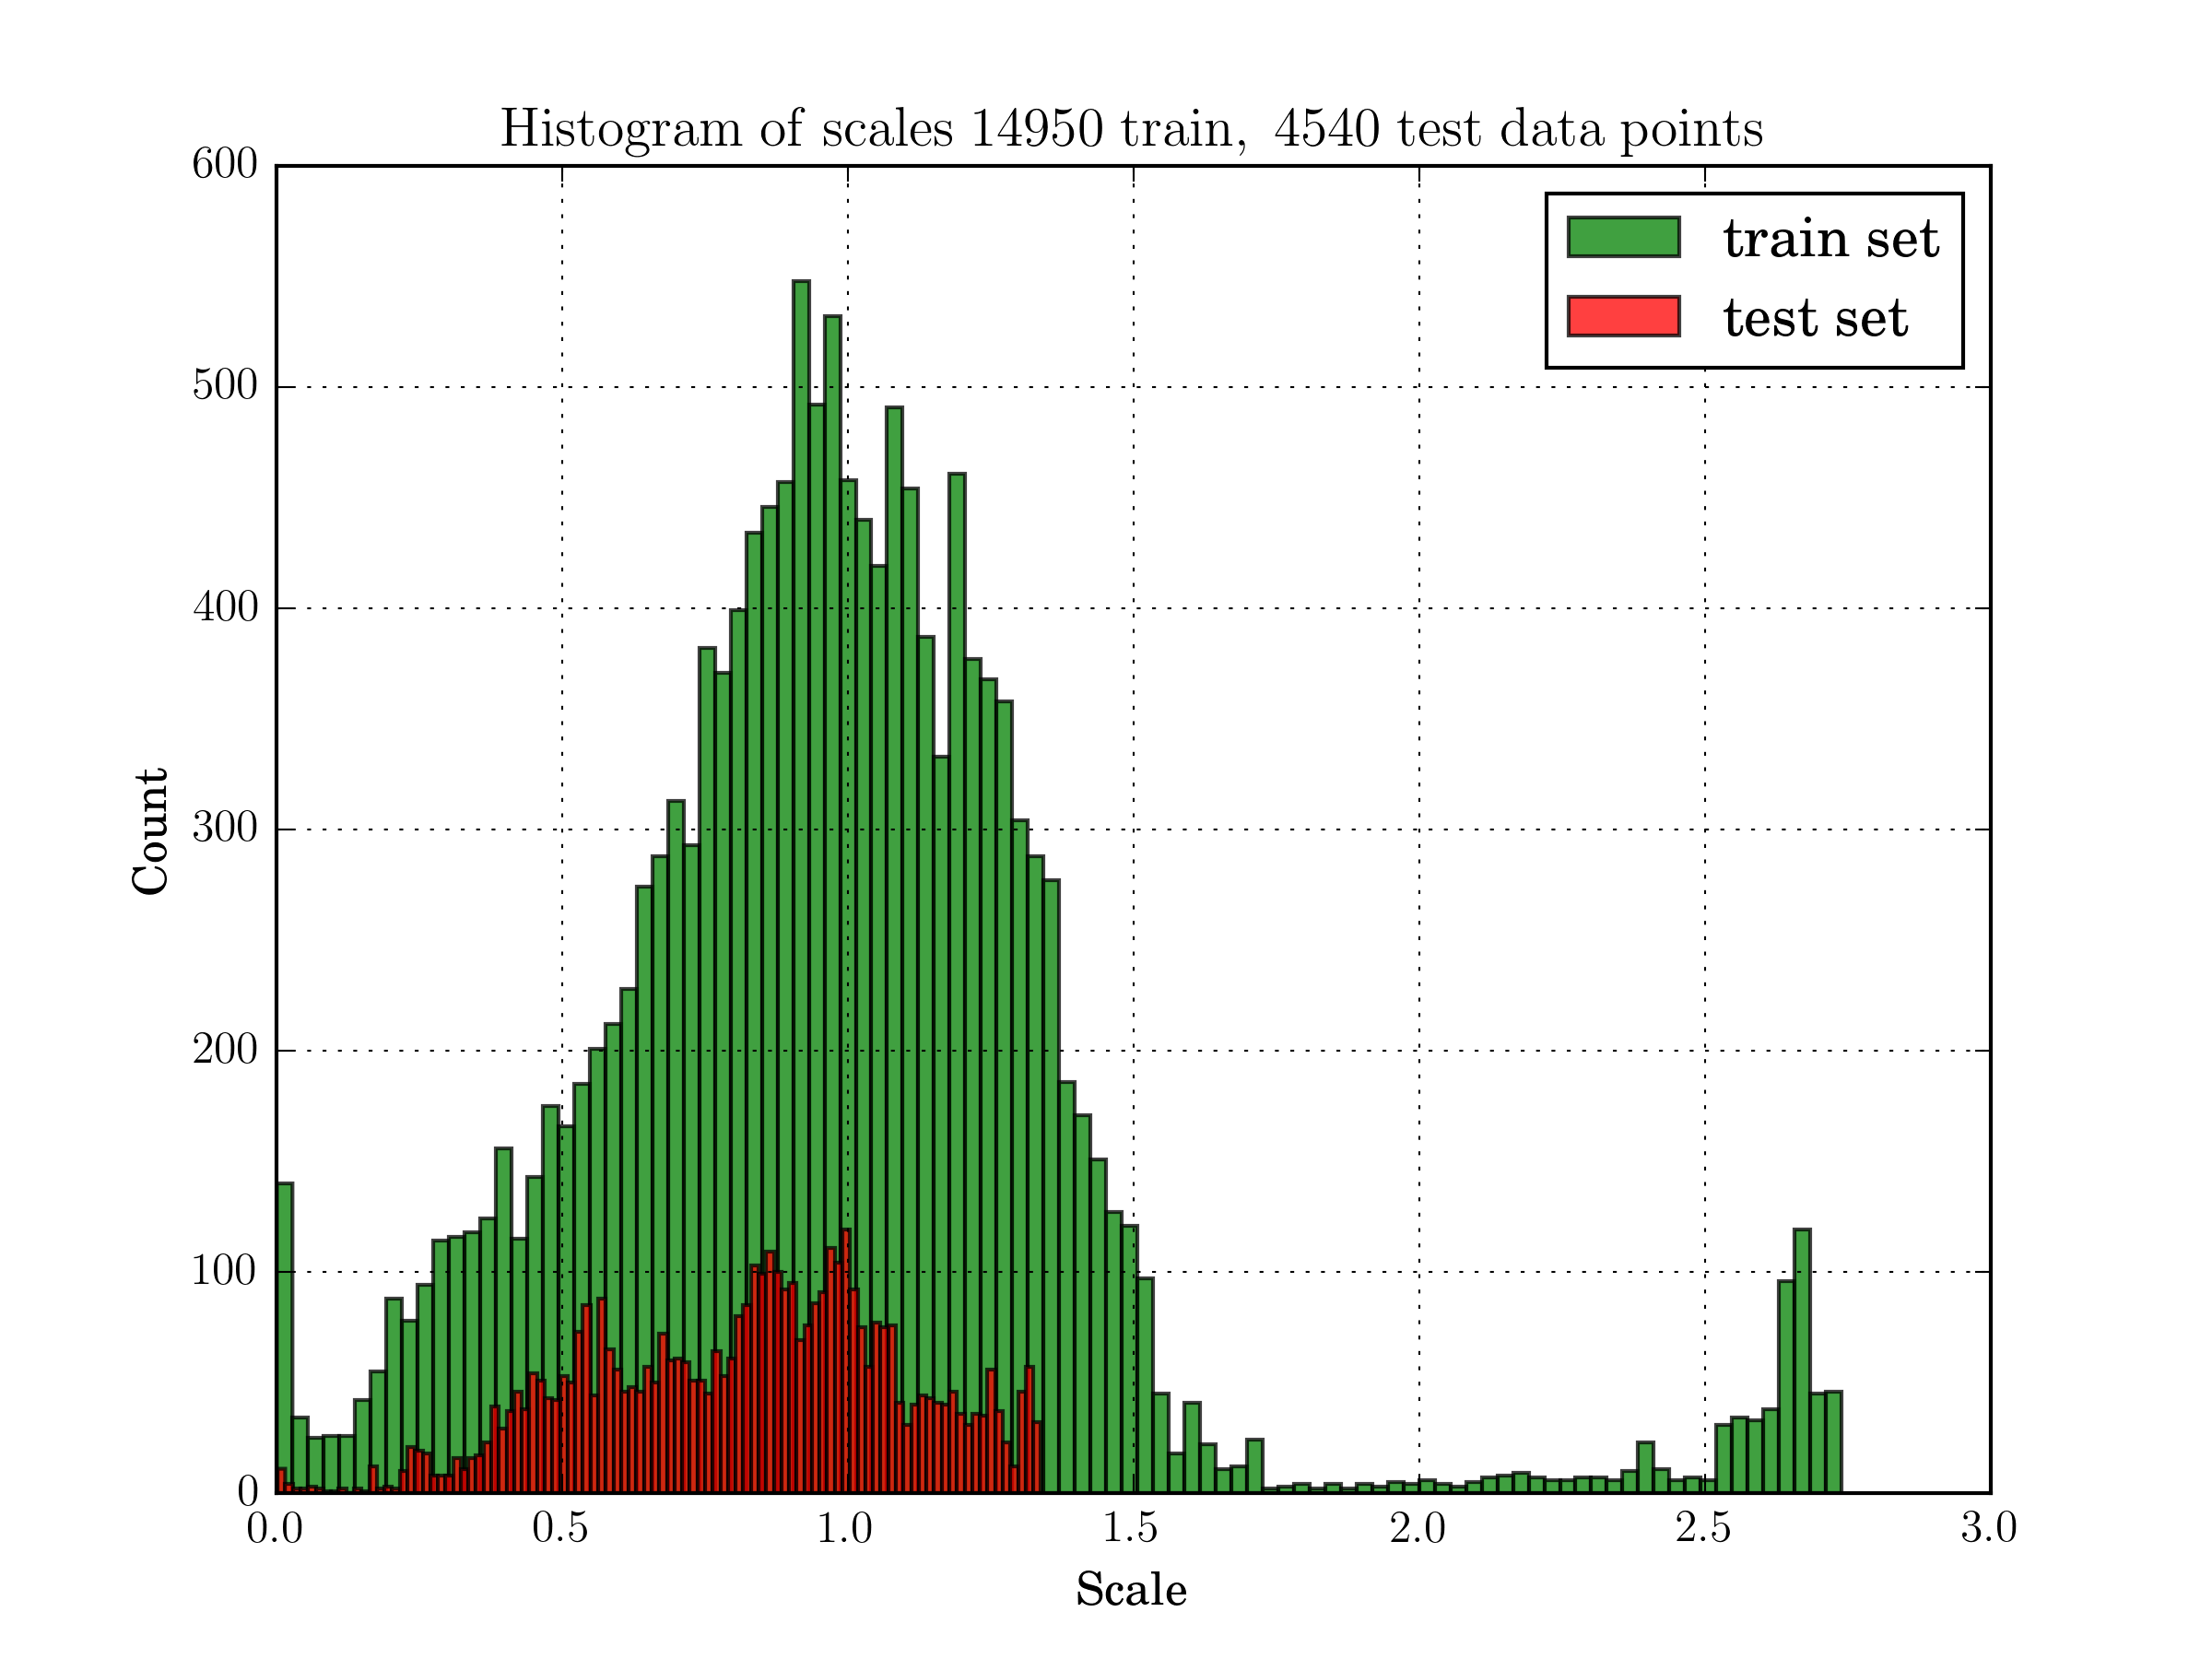
\includegraphics[width=0.9\linewidth]{no_00-scales}
  \caption{Scale distributions}
  \label{fig:scales}
\end{figure}

\subsection{Random Forest}\label{sec:features}

Training a random forest regressor requires hand crafted feature
extraction.  We convert subsequent image pairs to feature vectors as
follows: we extract and match sparse salient points in both input
images.  The output of this stage is a set of a corresponding pixel
locations.  For each salient feature we compute the spacial
displacement magnitudes (e.g., sparse optical flow).  We define a grid
in the image space and assign each salient point to a bin.  Next, we
create histogram of displacement magnitudes for each bin.
Concatenating all histograms together produces a feature vector. We
use Harris corners and square $11\times 11$ patches as corner
descriptors. Sum of square differences is used as a distance measure
with the winning pair declared a match.  To prune the outliers we fit
the fundamental matrix into the matched corner sets and remove the
corners that do not agree with the model.
Figure~\ref{fig:ex_corner_and_matching} shows a typical example of
extracted and matched corners.

Figure~\ref{fig:feature_vectors} depicts the statistics of the feature
vectors extracted from the training data. One can see the peaks, that
correspond to a closer image regions have a distributions shifted to
the right (i.e., larger displacements) and the peaks that correspond
to a regions farther away should be closer to zero.  This behavior can
be observed especially well for the feature vectors that correspond to
larger camera displacements (e.g. Figure~\ref{fig:1c}).  This figure
is an insight why we chose this particular type of feature vector: the
distribution of the displacements depends on the size of the camera
motion.

\begin{figure}[!ht]
  \centering
  \begin{subfigure}{.45\linewidth}
    \centering
    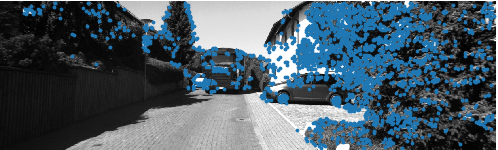
\includegraphics[width=\linewidth]{10_001157_001158_raw_corners_left}
    \caption{}
    \label{fig:ex_corner_and_matching:corner}
  \end{subfigure}
  \begin{subfigure}{.45\linewidth}
    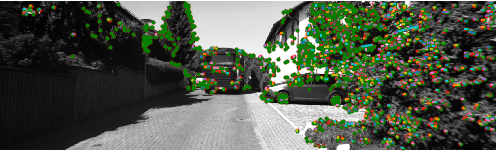
\includegraphics[width=\linewidth]{10_001157_001158_final_matches1}
    \caption{}
    \label{fig:ex_corner_and_matching:match}    
  \end{subfigure}
  \caption{Typical corner extraction and
    matching. Figure~\subref{fig:ex_corner_and_matching:corner} shows the raw
    extracted corners, while Figure~\subref{fig:ex_corner_and_matching:match} shows
    pruned and matched corners.}
  \label{fig:ex_corner_and_matching}
\end{figure}

\begin{figure}[!ht]
  \centering
  \begin{subfigure}{.45\linewidth}
    \centering
    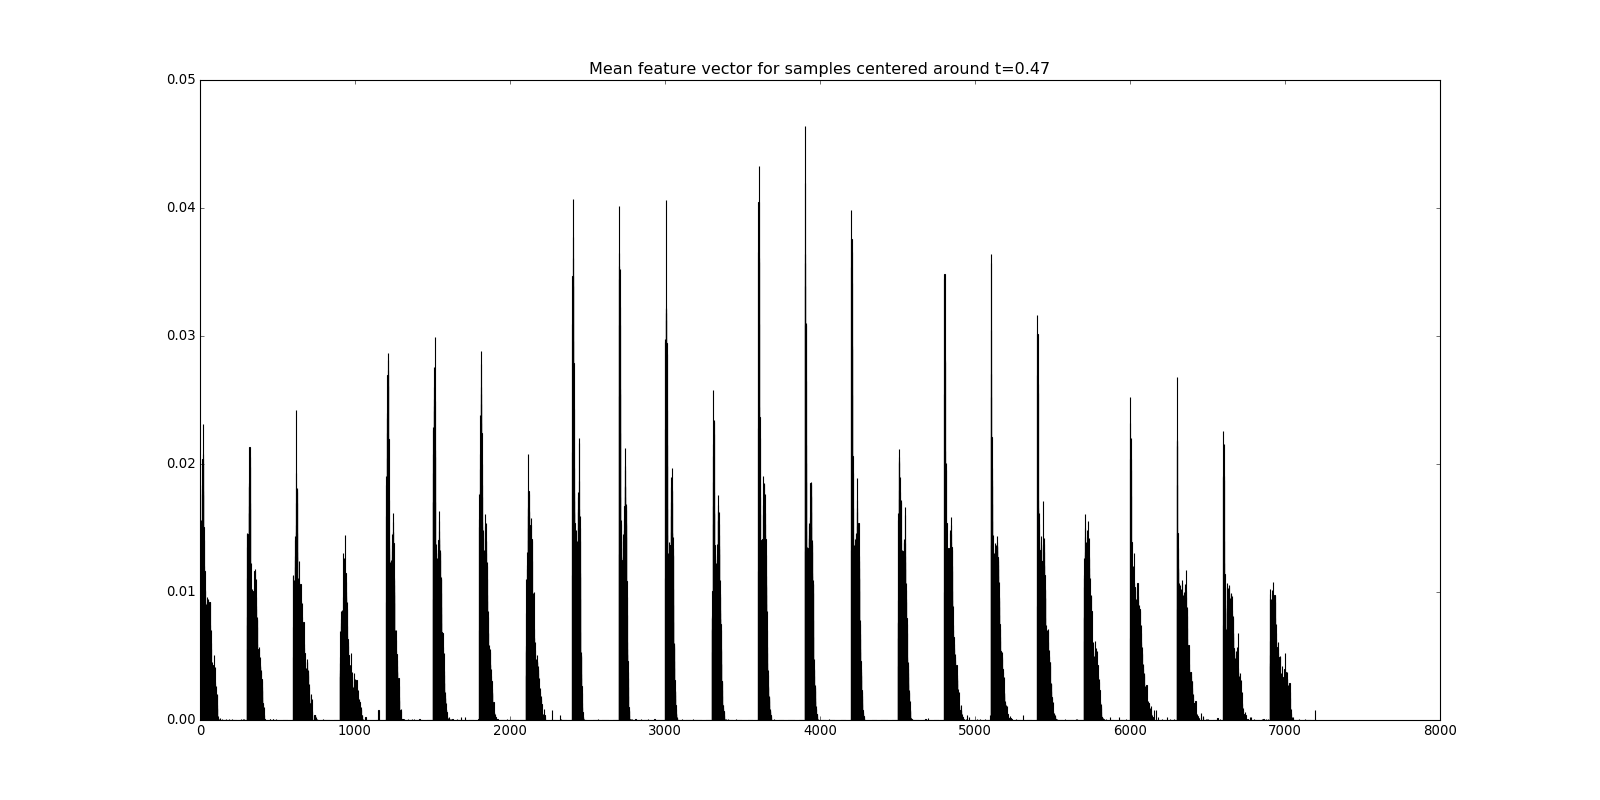
\includegraphics[width=1.2\linewidth]{00_mean_feature_vector_0_47}
    \caption{}\label{fig:1a}
  \end{subfigure}%
  \begin{subfigure}{.45\linewidth}
    \centering
    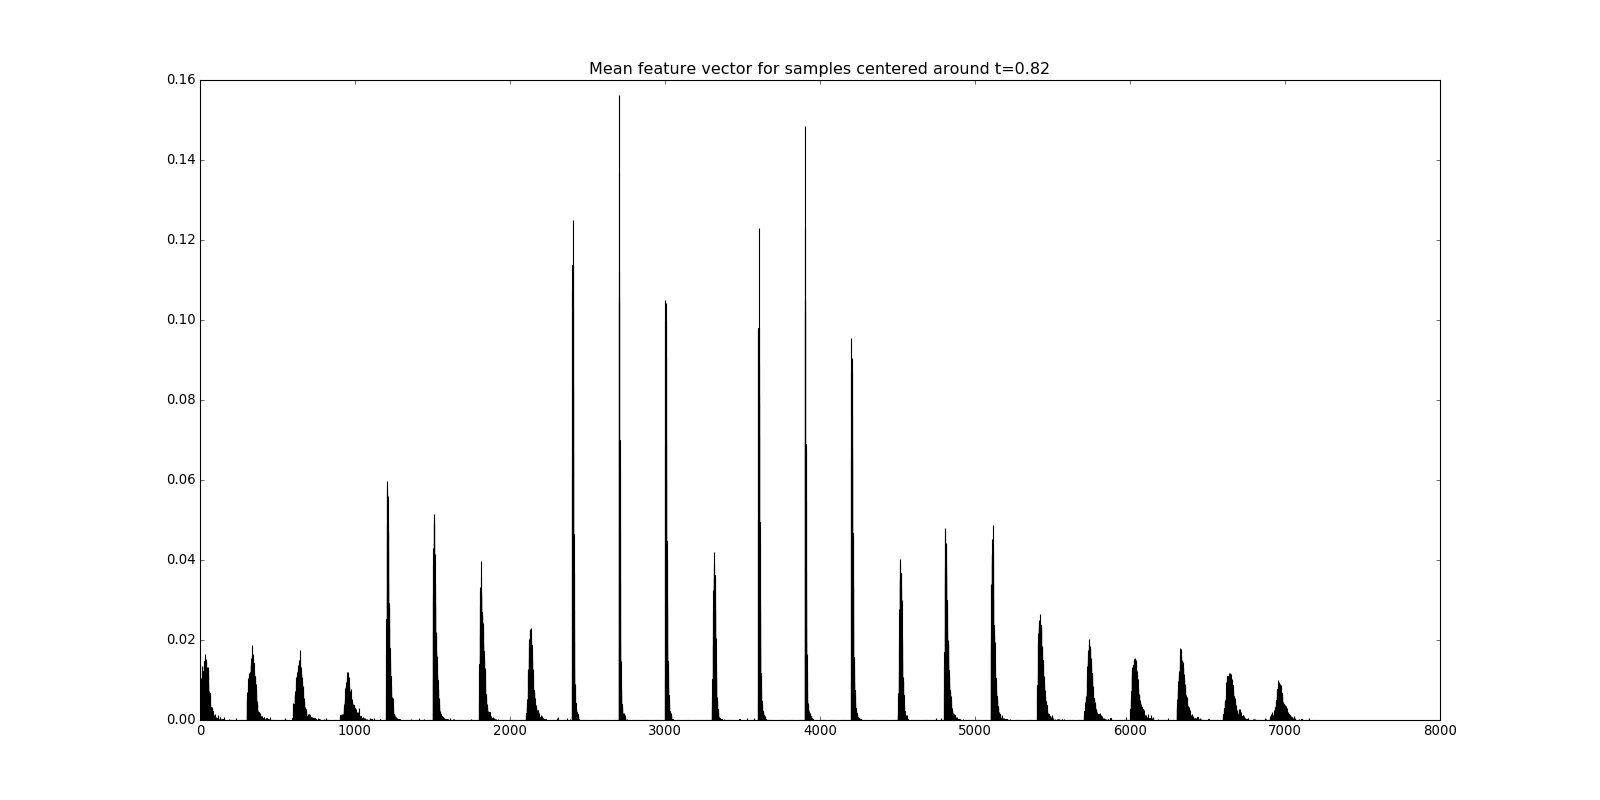
\includegraphics[width=1.2\linewidth]{00_mean_feature_vector_0_81}
    \caption{}\label{fig:1b}
  \end{subfigure}%
  \\
  \begin{subfigure}{\linewidth}
    \centering
    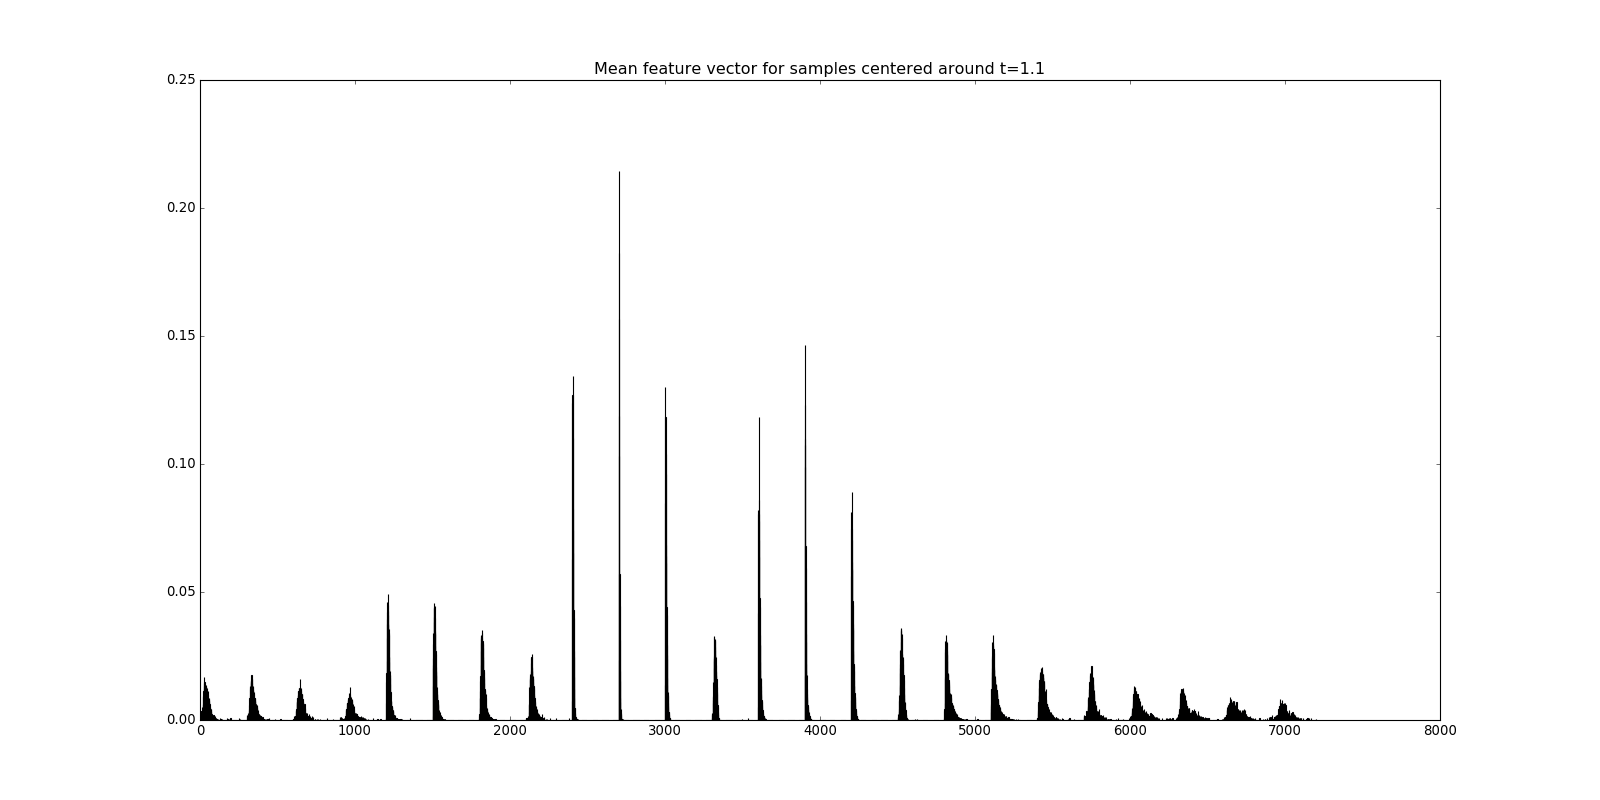
\includegraphics[width=.8\textwidth]{00_mean_feature_vector_1_1}
    \caption{}\label{fig:1c}
  \end{subfigure}%
  \caption{Average feature vectors (see~\protect\ref{sec:features})
    for samples centered around the specific camera translation
    magnitude.  Each peak corresponds to a grid cell (e.g., here the
    grid is 4 rows by 6 columns by 300 bins, so the feature vector has
    6*4*300=7200 dimensions).  The grid is sampled in a column-major
    mode. So the first four peaks correspond to the leftmost column of
    the image grid.}
  \label{fig:feature_vectors}
\end{figure}

We bin each image into $6\times 4$ grid.  For each bin in the image we
compute the histogram of corner disparities.  By disparity we denote
the displacement of the corner in the image.  We use $300$-bin
histogram for disparities (e.g, feature vector length is $7200$).  We
experimented with different values for the grid size, number of
histogram bins and number of random trees in the forest.
Aforementioned set of parameters was found empirically to give the
best results over the validation set.

We use the extracted features to fit a random forest of 100 trees, by
means of recursive node splitting with sub-node variance minimization.
We use scikit-lean~\cite{scikit-learn} random forest implementation.
As one may see in Table~\ref{table:train result}, random forest
exhibits a very low training error/variance but has weaker
generalization ability, as opposed to deep models.  One reason for
this may be that the features are not discriminative enough, i.e., the
feature vectors for two image pairs are very close while the scale of
the motion is distant.

See Section~\ref{sec:results} for random forest test inference
results.

\subsection{Neural networks}

We use Caffe~\cite{jia2014caffe} framework on a single NVIDIA Titan X
to train and test our models. For brevity, we elaborate on the
training details only for the FlowNet, since it attains best results.

\paragraph{ZF} We train using vanilla SGD for 100 epochs. Learning
rate is initialized to 1e-5 and decreases by factor of .1 every 10
epochs. We train the network from scratch.


\paragraph{FlowNet} We train using vanilla SGD for 100
epochs. Learning rate is initialized to 1e-5 and decreases by factor
of .1 every 10 epochs. We start from pre-trained weights
of~\cite{fischer2015flownet}. The training proceeds with mini-batch
size of 5. Train loss graph is shown in~\ref{fig:flownet_train_loss}.
It may be that we proceed with training after the loss stopped
decreasing, but it seems that 100 epoch training time is widely used
in the literature.  Also, note that the loss is periodic, which
happens because of multi-epoch training.  
\begin{figure}[!ht]
  \centering
  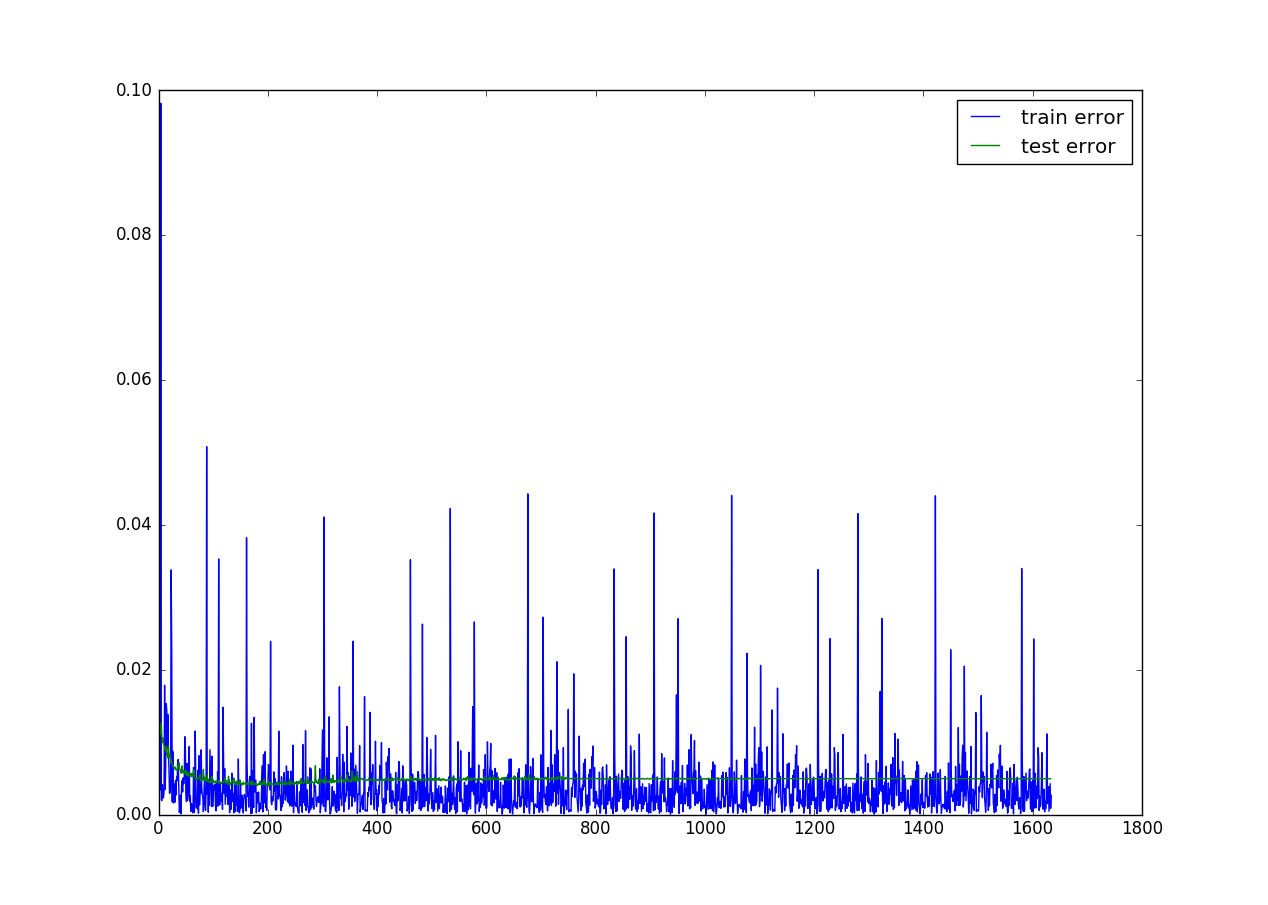
\includegraphics[width=0.9\linewidth]{losses}
  \caption{FlowNet train loss vs. test loss}
  \label{fig:flownet_train_loss}
\end{figure}

\paragraph{LSTM} We also train using vanilla SGD for 100 epochs
decreasing learning rate by .1 every 10 epochs.  We fine-tune from our
FlowNet trained CNN trained weights.

Table~\ref{table:train result} summarizes trained model error on the
training set.  This table shows that while random forest successfully
overfits the data, it has a limited generalization ability.

\begin{table}[ht]
  \centering
  \begin{tabular}{ lccccc }
    \hline
                       & Random Forest  & FlowNet       \\
    \hline
    $\mu_{abs}$        & 5.79e-06       & .056          \\
    $\sigma_{abs}$     & 1.40e-05       & .062          \\
    $\mu$              & 4.88e-15       & -2.28e-4      \\
    $\sigma$           & 1.51e-05       & .083          \\
    \hline
  \end{tabular}
  \caption{Training errors (in meters)}
  \label{table:train result}
\end{table}

\subsection{Results}\label{sec:results}

Let the ground truth sequence of camera motion scales be
$\{y_i\}_{i=1}^N$, the predicted scales for the same sequence be
$\{\hat{y}_i\}_{i=1}^N$, and the corresponding error sequence
$\{\delta_i\}_{i=1}^N$:
\begin{equation}
  \delta_i = y_i-\hat{y}_i,
\end{equation}

We report two results, the first one is a signed error mean similar to
the work of~\cite{frost2017using}:
\begin{equation}
  \mu = \frac{1}{N}\sum_{i=1}^N{\delta_i},
\end{equation}

The second result is the absolute error mean:
\begin{equation}
  \mu_{abs} = \frac{1}{N}\sum_{i=1}^N{|\delta_i|},
\end{equation}

The $\mu_{abs}$ and the $\sigma_{abs}$ show how close the estimates
are to the ground truth values.  The $\mu$ shows how biased the
estimator is.  We report corresponding standard deviations, as well,
in Table~\ref{table:main result}.  Best result in each category is
highlighted in bold.  FlowNet exhibits minimal absolute error and
lowest variance.  This is our model of choice.  Note that random
forest has best signed mean error, but is noisy.

\begin{table}[ht]
  \centering
  \begin{tabular}{ lccccc }
    \hline
                       & Random Forest     & ZF    & FlowNet          & LSTM FlowNet & \cite{frost2016}   \\
    \hline
    $\mu_{abs}$        & .237              & .200  & \textbf{.078}    & .097         & \\
    $\sigma_{abs}$     & .229              & .161  & \textbf{.061}    & .074         & \\
    $\mu$              & \textbf{-1.44e-3} & -.007 & .023             & .017         & .014\\
    $\sigma$           & .329              & .257  & \textbf{.098}    & .121         & .177\\
    \hline
  \end{tabular}
  \caption{Experimental Results (in meters)}
  \label{table:main result}
\end{table}

Our FlowNet produces predictions that have errors of lower variance
but are a bit less accurate than~\cite{frost2017using}.

Figure~\ref{fig:pred_vs_gt} and Figure~\ref{fig:rf_pred_vs_gt} shows
FlowNet and random forest scale predictions overlayed with the ground
truth values for the first 750 frames of the test sequence.  The
prediction is unbiased and noisy, clearly follows the trend of the
ground truth values.  Random Forest predictions are a lot more noisy
than those of the FlowNet.

\begin{figure}[!ht]
  \centering
  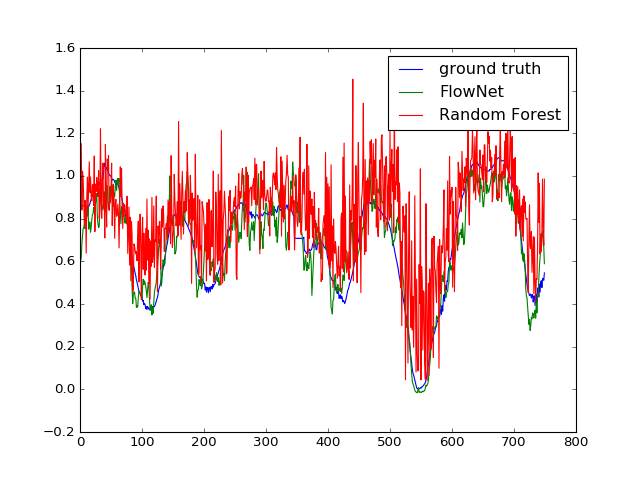
\includegraphics[width=0.9\linewidth]{flownet_prediction_vs_gt_vs_rf}
  \caption{FlowNet, Random Forest predictions vs. the ground truth}
  \label{fig:pred_vs_gt}
\end{figure}

\begin{figure}[!ht]
  \centering
  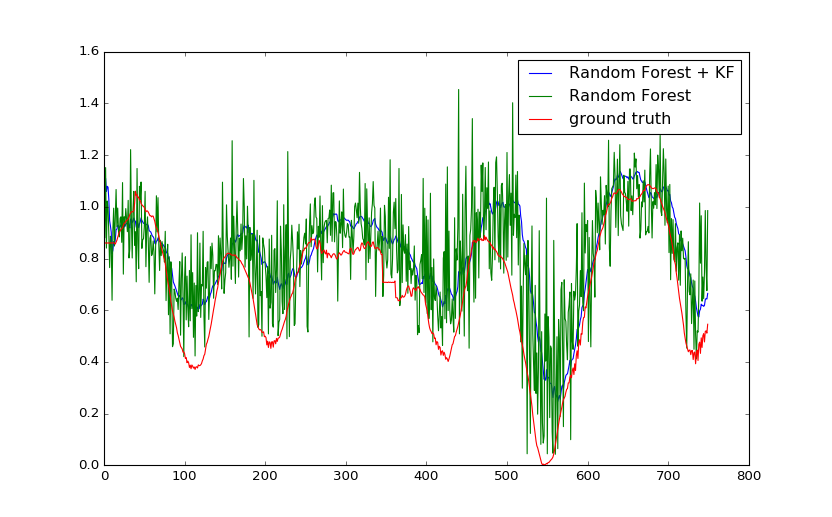
\includegraphics[width=0.9\linewidth]{rf_prediction_vs_gt}
  \caption{Random Forest prediction vs. ground truth}
  \label{fig:rf_pred_vs_gt}
\end{figure}

We perform an additional Kalman Filter step to smooth the predictions.
We use constant acceleration model.  To estimate the measurement and
the process noise we use sequence 02 as a validation set (see e.g.,
Figure~\ref{fig:02 stats}).  In this case the filter merely smoothes
the result and keeps the mean errors at the same level.  We do suggest
that at least for some trajectories the Kalman Filter may improve the
overall result, since it provides a physical constraint on camera
behavior.  The neural networks are known to give erroneous output when
the test data is far from the train data.  These are also the cases
where the filter may be beneficial.  The result of applying Kalman
Filter to both Random Forest and FlowNet predictions is in
Figure~\ref{fig:rf_pred_vs_gt_vs_ekf} and
Figure~\ref{fig:pred_vs_gt_vs_ekf_aug}, respectively.

\begin{figure}[!ht]
  \centering
  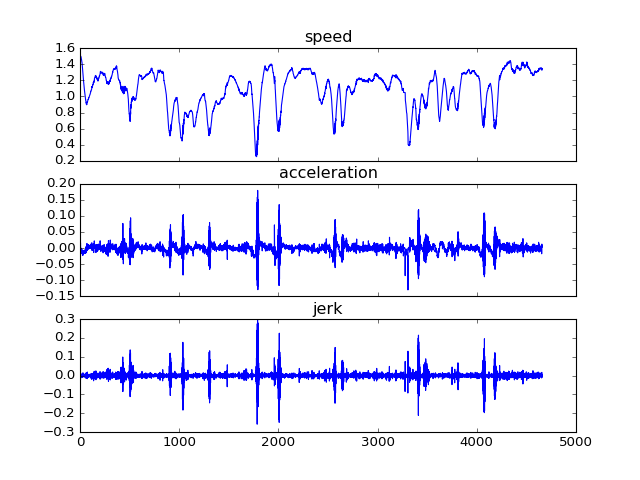
\includegraphics[width=0.9\linewidth]{02_speeds_accel_jerk}
  \caption{KITTI sequence 02 vehicle speed, acceleration and jerk}
  \label{fig:02 stats}
\end{figure}

\begin{figure}[!ht]
  \centering
  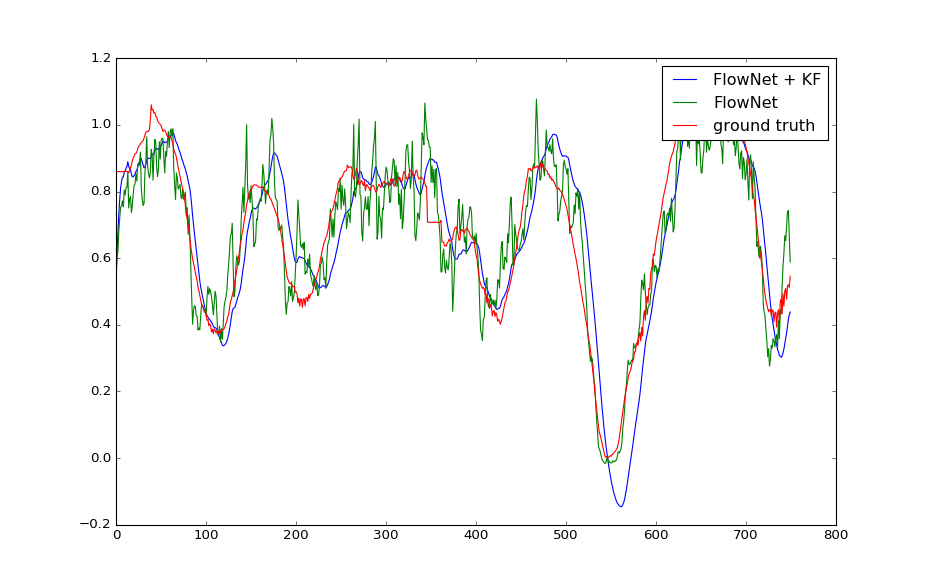
\includegraphics[width=0.9\linewidth]{flownet_prediction_vs_gt_vs_kf_aug}
  \caption{FlowNet prediction vs. ground truth vs. Kalman Filter}
  \label{fig:pred_vs_gt_vs_ekf_aug}
\end{figure}

\begin{figure}[!ht]
  \centering
  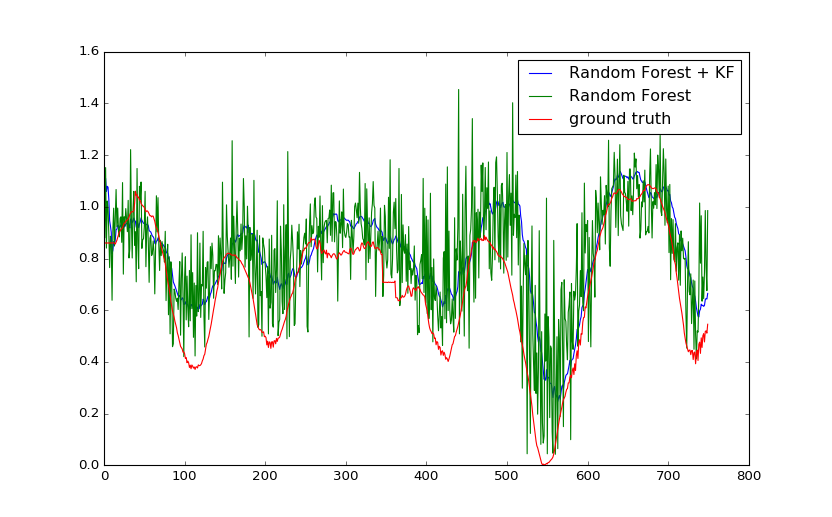
\includegraphics[width=0.9\linewidth]{rf_prediction_vs_gt_vs_kf}
  \caption{Random Forest prediction vs. ground truth vs. Kalman Filter}
  \label{fig:rf_pred_vs_gt_vs_ekf}
\end{figure}

Finally, we show how our scale affects motion estimation.  Let a
$N$-step path of a camera be described by a sequence of homogeneous
rigid poses $\{T_i\}_{i=0}^N$ as described in Section~\ref{sec:our
  method}.  In the current context each $T_i$ relates the $i$-th pose
of the camera to the beginning of the path (i.e., pose $T_0$).  Also,
denote the corresponding scale estimates by $\{s_i\}_{i=0}^N$.  We
construct a new path $\{\tilde{T}_i\}_{i=0}^N$ by re-scaling each
relative pose appropriately.

First we compute a pose that relates camera $i-1$ to camera $i$:
\begin{equation}\label{eq:delta T}
  \Delta T_i = T_{i-1}^{-1}T_i,
\end{equation}

We initialize a re-scaled relative pose to be identical to Eq.~\ref{eq:delta T}
\begin{equation}
  \Delta \tilde{T}_i = \Delta T,
\end{equation}

We re-scale the relative pose according to be the new scale (array
indexing follows Python numpy):
\begin{equation}
  \Delta \tilde{T}_i[:3,3] = s_i * \frac{\Delta T_i[:3,3]}{\norm{\Delta T_i[:3,3]}},
\end{equation}

Finally, we construct a new pose $\tilde{i}$:
\begin{equation}
  \tilde{T}_i = \tilde{T}_{i-1} * \Delta \tilde{T}_i,
\end{equation}

We use the above method to re-scale the ground truth 00 sequence path
according to raw scale estimation and a Kalman-smoothed one.  The
results are in Figure~\ref{fig:00_motion} and in
Figure~\ref{fig:00_motion_rf}.

\begin{figure}[!ht]
  \centering
  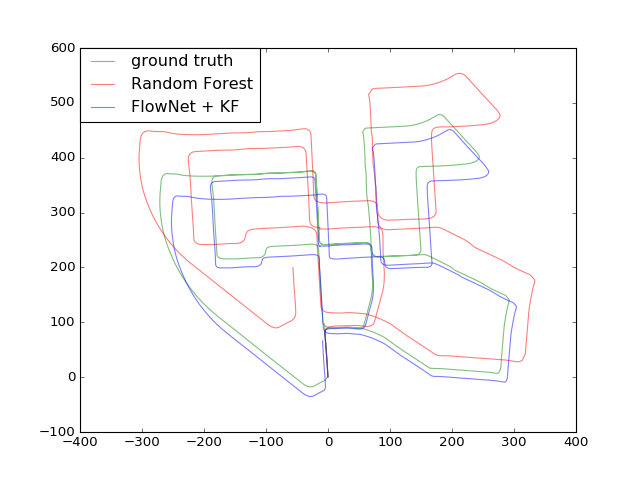
\includegraphics[width=0.9\linewidth]{00_motion_rf}
  \caption{Motion estimation, based on the Random Forest predictions}
  \label{fig:00_motion_rf}
\end{figure}

\begin{figure}[!ht]
  \centering
  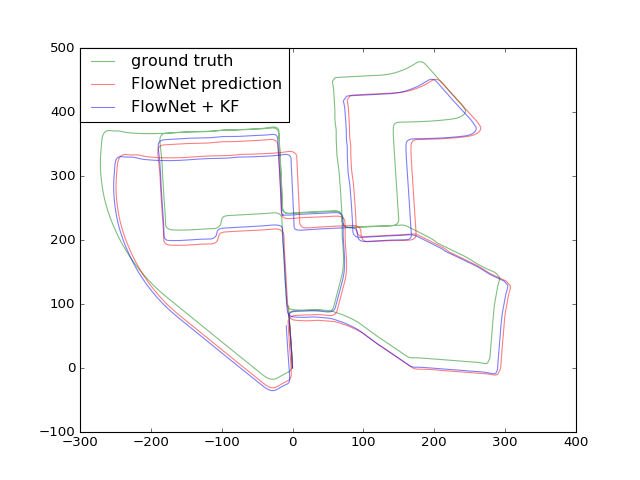
\includegraphics[width=0.9\linewidth]{00_motion_flownet}
  \caption{Motion estimation, based on the FlowNet predictions}
  \label{fig:00_motion}
\end{figure}

\section{Conclusions and Discussion}

This works presents a data driven approach for monocular scale
estimation.  We take a holistic path and learn the task end-to-end,
rather than splitting it into different sub-tasks.

We experimented with both ``shallow'' random-forest approach and more
recent deep learning methods.  Deep methods seem to outperform random
forest consistently.

We experiment with a number of deep architectures. We learned that the
fully convolutional architecture performs better than the traditional
(fully-connected layer based) networks.  The use of pre-trained weights
from the flow-network significantly improves the results.

The network performs about the same if trained on RGB or gray images.
We explored different ways for data augmentation, e.g, train the
network on images of the right camera as well as the left camera,
train on image pairs that are not strictly subsequent, but did not
find significant improvement.

Our results show that statistical machine learning is a viable
candidate for monocular scale estimation.  The (independent) work
of~\cite{frost2017using} also shows that it may be used to produce scale
drift free reconstructions.  These methods have a benefit of not-making
scene, camera pose assumptions, which may render them as more widely
applicable in the future.  In this work we deliberately did no scale
refinement or blending with other scale estimation methods, to show
clearly what the convnets are capable of in this specific context.

Surprisingly, LSTM did not do better than convnets, which is against
our expectations. The reason may be that we did not find a proper way
to train it.

The main challenge is how to go beyond a purely supervised approach
and better utilize the abundance of information that is present in the
images to get better predictions.

%%% Local Variables:
%%% mode: latex
%%% TeX-master: "../thesis"
%%% End:
